\section{Логика работы программы} \label{logic}
\subsection{Структурирование программы по Задачам}
Работа СПО «Кама-Надир» структурирована по решаемым задачам согласно  схеме на Рис.~\ref{fig:general_scheme}.
\begin{figure}[H]
    \centering
    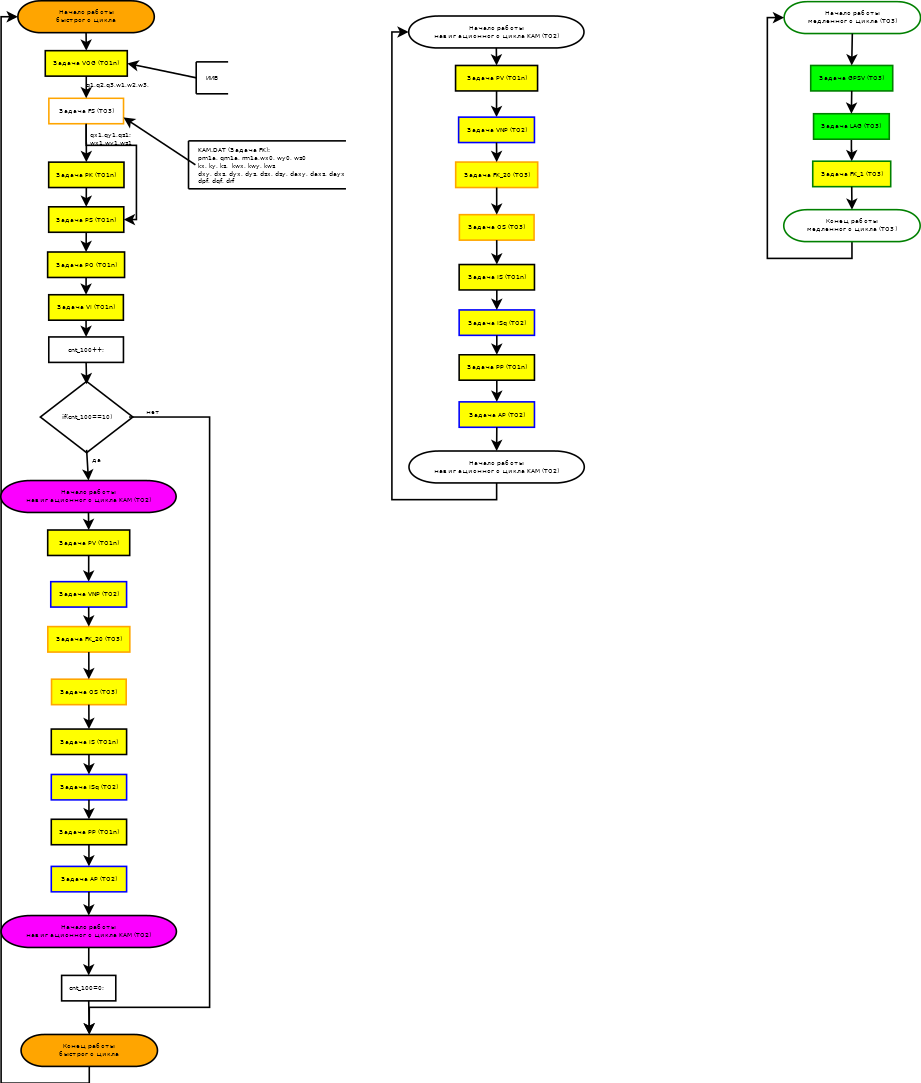
\includegraphics[width=1.0\linewidth]{images/general_scheme.png}
    \caption{Задачи программы}
    \label{fig:general_scheme}
\end{figure}
\subsection{Задача формирования сигналов FS}
Реализует следующие функции согласно схеме на Рис.~\ref{fig:FS}
\begin{figure}[H]
    \centering
    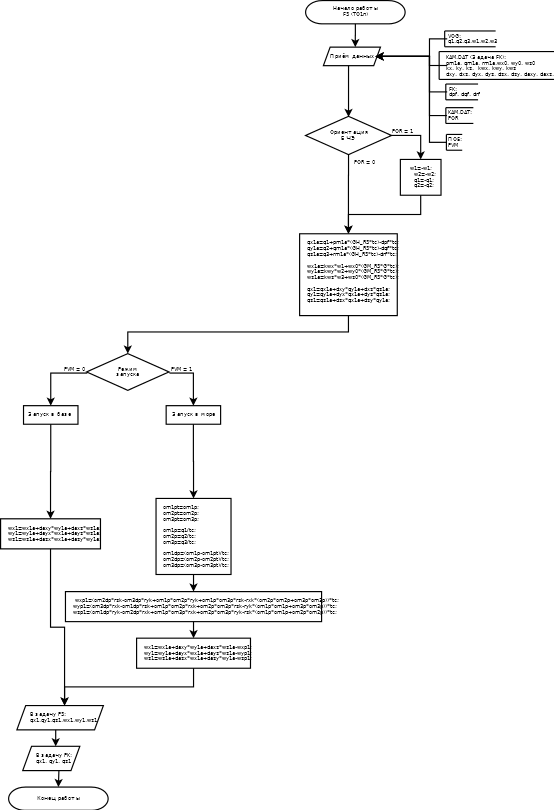
\includegraphics[width=0.8\linewidth]{images/FS.png}
    \caption{Задача FS}
    \label{fig:FS}
\end{figure}
\begin{itemize}
\item Принимает от задачи VOG сигналы - q1,q2,q3,w1,w2,w3 и формирует с учетом принятой модели  инструментальных погрешностей передаваемые в задачи PK и PS  
приращения угла поворота qx1,qy1,qz1 и кажущейся скорости wx1,wy1,wz1 в проекциях на оси БЧЭ.
\item Преобразует сигналы горизонтных каналов ВОГ- q1,q2  к осям обьекта при значении признака ориентации POR=1 в случае установки корпуса БЧЭ 
с поворотом на 180 относительно продольной оси объекта.
\item Осуществляет масштабирование, компенсацию аддитивных и мультипликативных составляющих модели  инструментальных погрешностей   
сигналов ВОГ и акселерометров с использованием задаваемых в случае необходимости в файле данных KAM.DAT корректур, а также меняющихся в запуске 
и  оцениваемых оптимальным фильтром Калмана ( ОФК ) составляющих дрейфов в осях БЧЭ:  
    \begin{itemize}
\item систематических ошибок  pm1a, qm1a, rm1a,wx0, wy0, wz0
\item масштабных коэффициентов kx, ky, kz,  kwx, kwy, kwz
\item невыставок  dxy, dxz, dyx, dyz, dzx, dzy, dаxy, dаxz, dаyx
\item оценки дрейфов dpf, dqf, drf
    \end{itemize}
\end{itemize}
\subsubsection{Входные и выходные данные задачи FS}
Входная информация
\begin{itemize}
    \item q1, q2, q3, w1,w2,w3- из задачи  VOG-приема сигналов БЧЭ
    \item pm1a,qm1a, rm1a, wx0, wy0, wz0, kwx, kwy, kwz, dxy, dxz, dyx, dyz, dzx, dzy, daxy, daxz, dayx, dayz, dazx, dazy - из файла данных kam.dat
    \item dpf, dqf, drf- из задачи  FK
\end{itemize}
Выходная информация
\begin{itemize}
    \item qx1, qy1, qz1- в задачу PK
    \item qx1,qy1,qz1,wx1,wy1,wz1-- в задачу PS
\end{itemize}
\subsection{Задача формирования скоростей опорного трехгранника OS}
Реализует следующие функции согласно упрощенной схеме на Рис.~\ref{fig:OS}
\begin{figure}[H]
    \centering
    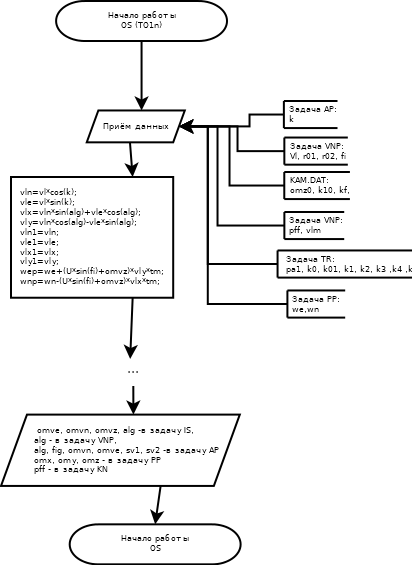
\includegraphics[width=0.8\linewidth]{images/OS_simple.png}
    \caption{Задача OS}
    \label{fig:OS}
\end{figure}
\begin{itemize}
    \item Формирует угловую скорость коррекции $\omega$  ( omx ,  omy,  omz ) -составляющие   угловой скорости   опорного   аналитического   
    трехгранника в проекциях  на собственные оси  - 
    по информации из задачи  PV о проекциях на горизонтальную плоскость аналитического трехгранника  приращения  кажущейся скорости БИНС 
    в осях аналитического  опорного трехгранника  за время  навигационного  цикла  ТМ.-- Wг (We, Wn, Wv).  
    \item Вычисляет по сигналу лага  VL  горизонтальные  составляющие скорости   обьекта в  проекциях  на оси  географического трехгранника VLE, 
    VLN с использованием курса К и -на оси  опорного   аналитического   трехгранника  VLX,  VLY с использованием курсового  угла  ALG 
    \item Компенсирует в  горизонтальных проекциях сигналов акселерометров кориолиссовы составляющие,  порождаемые вертикальной составляющей угловой 
    скорости  опорного   аналитического   трехгранника $omvz=U*sin(\phi)$  и  горизонтальными  составляющими скорости   обьекта в проекциях  на 
    оси  опорного   аналитического   трехгранника  для получения после их интегрирования  только составляющих скорости относительно Земли и  
    сравнения их с составляющими  сигнала  лага  в проекциях  на оси  опорного   аналитического   трехгранника   на предыдущем  шаге  
    VLX1,  VLY1  с  целью  формирования сигналов демпфирования   sv1,   sv2.
    \item В рабочем режиме (pa1=3) формирование сигналов демпфирования  sv1, sv2 и  абсолютных угловых скоростей опорного  аналитического  трехгранника  
    omve,  omvn,   omvz  производится  c  использованием корректур  dvx,   dvy,  выработанных  ОФК .
    \item Формирование  составляющих угловой скорости опорного   аналитического  трехгранника в проекциях  на собственные оси - выходные сигналы 
    задачи   OS-производится  с использованием корректур  db,   dg,   dalf,   выработанных  ОФК, что также обеспечивает демпфирование переходных 
    процессов, вызванных реальными начальными угловыми рассогласованиями , начальными отклонениями угловых скоростей, 
    ускорениями качки и инструментальными погрешностями.
    \item В конце задачи реализуется   контроль  уровня  угловых скоростей опорного трехгранника  и в случае  превышения  горизонтальными составляющими 
    угловых скоростей omx  или  omy  значения 2-4  рад/сек  (60  град/час)  включается счетчик циклов  cnf.
\end{itemize}
\subsubsection{Входные и выходные данные задачи OS}
Входная информация:
\begin{itemize}
    \item Vl, r01, r02, fi - из задачи  VNP
    \item pa1, k0, k01, k1, k2, k3 ,k4 ,k5 - из задачи   TR
    \item we,wn- из задачи   PP
    \item omz0, k10, kf, -из файла данных kam.dat
    \item k -из задачи AP
\end{itemize}
Выходная информация:
\begin{itemize}
\item omve, omvn, omvz, alg -в задачу IS, 
\item alg - в задачу VNP,
\item alg, fig, omvn, omve, sv1, sv2 -в задачу AP
\item omx, omy, omz - в задачу PP
\item pff - в задачу KN
\end{itemize}
\subsection{Задача вычисления параметров кватерниона РК}
Вычисляет, согласно упрощенной схеме на Рис.~\ref{fig:PK},  по  информации о приращениях за время быстрого цикла ТC  абсолютного угла поворота $\delta$ Q в проекциях на оси БЧЭ -  qx1, qy1, qz1, - из задачи  FS 
компоненты кватерниона mm (m0m, m1m, m2m, m3m), определяющего  ориентацию связанных осей БИНС относительно инерциального трехгранника путем численного 
интегрирования кинематического уравнения Пуассона.
\begin{figure}[H]
    \centering
    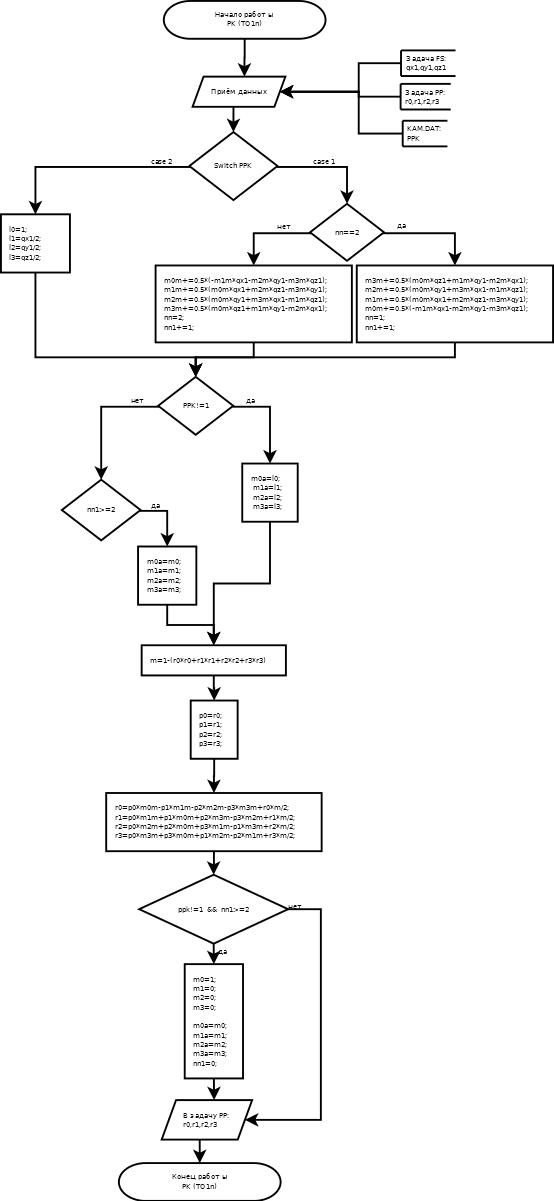
\includegraphics[width=0.5\linewidth]{images/PK.png}
    \caption{Задача PK}
    \label{fig:PK}
\end{figure}
\subsubsection{Входные и выходные данные задачи РК}
Входная информация:
\begin{itemize}
\item qx1,qy1,qz1- из задачи  FS
\item r0,r1,r2,r3- из задачи  PP
\item ppk- из файла данных kam.dat
\end{itemize}
Выходная информация:
\begin{itemize}
    \item r0,r1,r2,r3- в задачу PP
\end{itemize}
\subsection{Задача определения параметров ориентации PO}
Вычисляет, согласно упрощенной схеме на Рис.~\ref{fig:PO}, курс и углы бортовой и килевой качек БИНС –kbv,  tbv,  pbv,  
а  также скорости изменения курса и углов бортовой и килевой качек –kbvt,  tbvt,  pbvt  по  информации о компонентах кватерниона  r 
из задачи РР,  курсовому углу опорного трехгранника АLF из  задачи IS или,  в случае режима приведения, по  углу  ALG из  задачи  OS, 
вычисляемого методом гирошироткомпаса.
\begin{figure}[H]
    \centering
    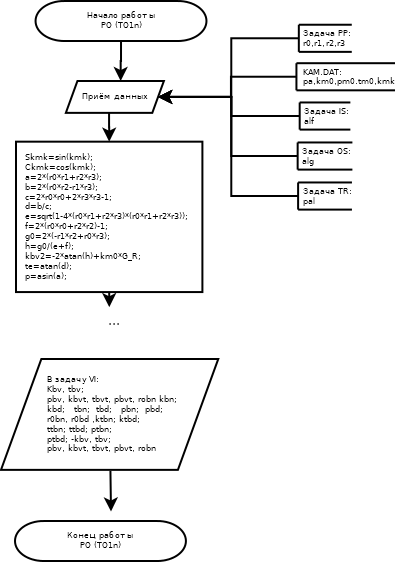
\includegraphics[width=0.5\linewidth]{images/PO_simple.png}
    \caption{Задача PO}
    \label{fig:PO}
\end{figure}
\subsubsection{Входные и выходные данные задачи РО}
Входная информация:
\begin{itemize}
\item r0,r1,r2,r3- из задачи  РР
\item pa,km0,pm0.tm0,kmk- из файла данных kam.dat
\item alf- из задачи  IS
\item alg- из задачи  OS
\item pa1- из задачи  TR
\end{itemize}
Выходная информация:
\begin{itemize}
    \item Kbv, tbv; pbv, kbvt, tbvt, pbvt,robn kbn; kbd;   tbn;  tbd;   pbn;  pbd; r0bn,   
    r0bd ,ktbn; ktbd; ttbn; ttbd; ptbn; ptbd;-kbv, tbv; pbv, kbvt, tbvt, pbvt, robn - в задачу VI
\end{itemize}
\subsection{Задача преобразования скоростей PS}
Вычисляет, согласно схеме на Рис.~\ref{fig:PS}, по  информации о приращениях  абсолютного угла поворота и кажущейся скорости  qx1, qy1, qz1, wx1, wy1, wz1 - 
из задачи  FS  приращениях   кажущейся скорости  w1x, w1y, w1z  
в осях связанного трехгранника путем численного интегрирования кинематического уравнения для  производной вектора абсолютной скорости V  
во вращающихся c абсолютной  угловой скоростью $\omega$  осях.
\begin{figure}[H]
    \centering
    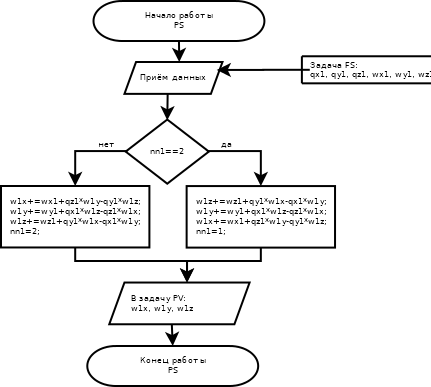
\includegraphics[width=0.5\linewidth]{images/PS.png}
    \caption{Задача PS}
    \label{fig:PS}
\end{figure}
\subsubsection{Входные и выходные данные задачи PS}
Входная информация:
\begin{itemize}
\item qx1, qy1, qz1, wx1, wy1, wz1 из задачи  FS
\end{itemize}
Выходная информация:
\begin{itemize}
    \item w1x, w1y, w1z в задачу PV
\end{itemize}
\subsection{Задача перепроектирования скоростей PV}
Перепроектирует согласно схеме на Рис.~\ref{fig:PV} приращения  кажущейся скорости БИНС  w ( w1x, w1y, w1z)  
в осях связанного трехгранника  за время  навигационного  цикла  ТМ  на  горизонтальную плоскость аналитического  опорного трехгранника 
с использованием кватерниона  r ( r0,  r1,  r2,  r3).
\begin{figure}[H]
    \centering
    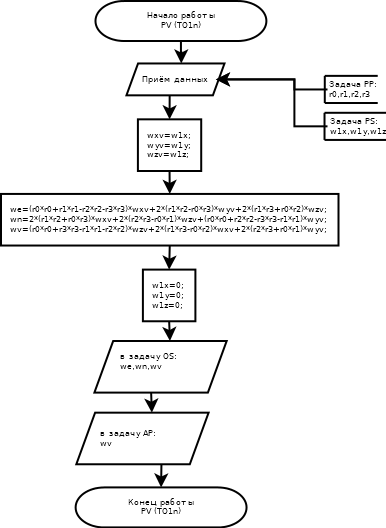
\includegraphics[width=0.5\linewidth]{images/PV.png}
    \caption{Задача PV}
    \label{fig:PV}
\end{figure}
\subsubsection{Входные и выходные данные задачи PV}
Входная информация:
\begin{itemize}
\item r0,r1,r2,r3- из задачи  РP
\item w1x,w1y,w1z- из задачи  РS 
\end{itemize}
Выходная информация:
\begin{itemize}
\item we,wn,wv- в задачу OS
\item wv- в задачу AP
\end{itemize}
\subsection{Задача выработки массива выходной информации VI}
Реализует следующие функции согласно схеме на Рисунок 8:
\begin{figure}[H]
    \centering
    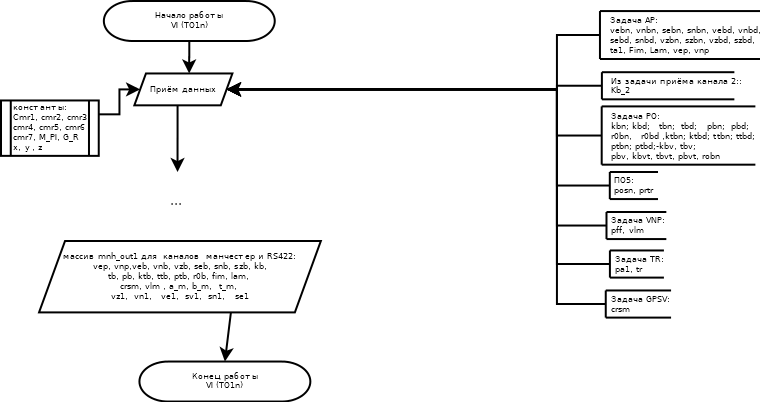
\includegraphics[width=0.75\linewidth]{images/VI_simple.png}
    \caption{Задача VI}
    \label{fig:VI}
\end{figure}
\begin{itemize}
    \item Определяет интервал времени RES  между текущим моментом и  моментом формирования экстраполяционных  коэффициентов в  задаче АР \\
RES = ElapsedTime(T);  \ время между текущим моментом  и моментом формирования \\
            qb1 = Res/0.1+q0;   параметров   Vbn …szbd в задаче аппроксимации, \\
            q0 = 0;             решаемой с циклом 0.1 сек \\
    \item Определяет   интервал времени  RES1  между текущим моментом  и  моментом формирования экстраполяционных  коэффициентов в  задаче   РO 
RES1 = ElapsedTime(T);  \ время между текущим моментом и моментом формирования \\
            qb2 = Res1/0.01+q0;       \ параметров  kbn   ptbd в задаче PO решаемой с циклом 0.01 сек
    \item Осуществляет  линейную  экстраполяцию  выходных  значений  составляющих  мгновенной скорости  VEB,  VNB, VZB  и  перемещений  
    SEB,  SNB,  SZB  c  использованием экстраполяционного сдвига q1  и  коэффициентов   линейной  экстраполяции vebn, vnbn, vzbn, sebn, snbn, szbn, 
    vebd, vnbd, vzbd, sebd, snbd, szbd   из задачи АР
    \item Осуществляет  линейную  экстраполяцию  выходных  значений углов  ориентации  kbv,  tbv,  pbv  и угла наклона  rob  и  
    угловых скоростей  ориентации kbt,  tbt,  pbt c  использованием экстраполяционного сдвига   q2  и  коэффициентов   линейной 
    экстраполяции      kbn;   kbd;   tbn;   tbd;   pbn;   pbd;    r0bn,   r0bd , ktbn;  ktbd;  ttbn;   ttbd;  ptbn;   ptbd     
    из задачи РО   в  случае,  когдазадача VI  решается  с  большей  частотой,  чем   РО 
    \item Осуществляет преобразование мгновенных скоростей veb, vnb, vzb и перемещений   seb, snb, szb от места установки БИНС  (т.О) 
    до места установки потребителя (т.П) с использованием проекций (x, y, z) отстояния R1 в связанных с БИНС  осях XYZ 
\end{itemize}
\subsubsection{Входные и выходные данные задачи VI}
Входная информация:    
\begin{itemize}
\item $vebn, vnbn, sebn, snbn, vebd, vnbd, sebd, snbd, vzbn, szbn, vzbd, szbd, ta1, Fim, Lam, vep, vnp$ – из задачи АР
\item $kbn; kbd;   tbn;  tbd;   pbn;  pbd; r0bn,   r0bd ,ktbn; ktbd; ttbn; ttbd; ptbn; ptbd;-kbv, tbv; pbv, kbvt, tbvt, pbvt, robn$– из задачи PO
\item $Kb_2$ -из задачи приема информации 2 канала
\item $posn, prtr$-c  пульта оператора
\item $pff, vlm$ - из задачи VNP
\item pa1, tr- из задачи TR
\item crsm - из задачи GPSV-прием СНС
\end{itemize}
Выходная информация:
\begin{itemize}
    \item массив mnh_out1,   содержащий выходные параметры $vep, vnp, veb, vnb, vzb, seb, snb, szb, kb, tb, pb, ktb, ttb, ptb, r0b, fim, lam, crsm, vlm , 
    a_m, b_m,  t_m, vz1,  vn1,   ve1,  sv1,  sn1,   se1$   – для  каналов  манчестер и RS422
\end{itemize}
\subsection{Задача коррекции положения опорного трехгранника РР}
Осуществляет, согласно схеме на Рис.~\ref{fig:PP}, коррекцию  кватерниона r ,  определяющего ориентации связанного трехгранника относительно  
аналитического опорного трехгранника с использованием  кватерниона  поворота опорного аналитического трехгранника   относительно   
инерциального трехгранника  S  (  S1,  S2,  S3 ) за время навигационного  цикла  ТМ c  помощью  формулы кватернионного произведения.
\begin{figure}[H]
    \centering
    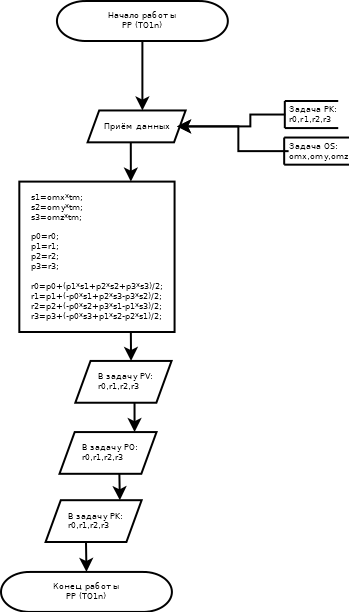
\includegraphics[width=0.75\linewidth]{images/PP.png}
    \caption{Задача PP}
    \label{fig:PP}
\end{figure}
\subsubsection{Входные и выходные данные задачи РР}
Входная информация:
\begin{itemize}
 \item r0,r1,r2,r3- из задачи  РК
 \item omx,omy,omz - из задачи  OS
\end{itemize}
Выходная информация:
\begin{itemize}
\item r0,r1,r2,r3- в задачу PV, PO,PK
\end{itemize}
\subsection{Задача инерциального счисления IS}
Реализует следующие функции согласно упрощенной схеме на Рис.~\ref{fig:IS}:
\begin{itemize}
    \item при включении (sgn1==0) проводит инициализацию переменных:  координат  fii,   lai:
    \begin{itemize}
        \item при отказе или отсутствии ПА СНС (prgk=0) значениями записанными в файл данных  kam.dat через задачу TR   fii=fiv;   lai=lav;
        \item при годности ПА СНС (prgk=1) значениями,  полученными от корабельной ПА СНС    fii=fivkg; lai=lavkg;
        \item при включении после режима Квази ( sgn2==0 ) значениями  координат,  пересчитанными в задаче Квази из квазигеографической в географическую систему координат fii=fiiqp;     lai=laiqp;
курсового угла  alf
        \item при  обычном запуске значением  курсового угла  alg  из задачи OS, определенным методом гирошироткомпаса  в режиме приведения   alf=alg; 
        \item при запуске в технологическом  режиме  гирогоризонткомпаса( pa=0)  нулевым значением  курсового угла  alf=0;
        \item при  повторном включении после перезапуска ПА СНС ( przv==3 ) значением курсового угла  alf1,  сохраненного в задаче VNP 
        в момент выключения задачи  IS для восстановления его значения  -alf=alf1;
        -при включении после режима Квази ( sgn2==0 ) значением  курсового угла,  пересчитанными в задаче Квази из квазигеографической 
        в географическую систему координат alf=alfqp;  
        \item параметра  rmk2,  определяющего скорость вращения опорного трехгранника в азимуте;
        \item при работе в обычных режимах  ( pa=1) значением  omvz  из задачи  OS  rmk2=omvz ;  
        \item при работе в технологическом  режиме  гирогоризонткомпса  ( pa=0) значением  вертикальной составляющей 
        угловой скорости ГСК $mk2=U*sin(\phi)+vle*tan(\phi)/r01$, формируемой по информации о широте fi и скорости от лага vl из задачи VNP;
    \end{itemize}
    \item Обнуляет  параметры  Sign1, sign2  для последующих  перезапусков  и  скорость  демпфирования  oz1k  в текущем запуске 
    \item формирует выражения для  интегрирования значений географической широты  fii, долготы lai,  и курсового угла alf.
\end{itemize}
\begin{figure}[H]
    \centering
    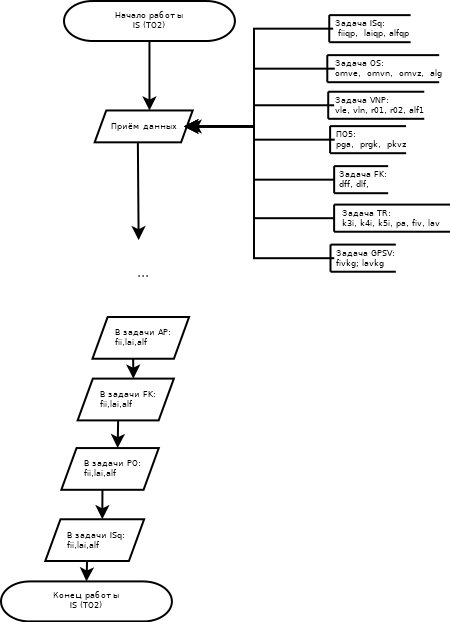
\includegraphics[width=0.75\linewidth]{images/IS_simple.png}
    \caption{Задача IS}
    \label{fig:IS}
\end{figure}


